% "{'classe':('PSI'),'chapitre':'slci_stabilite','type':('td'),'titre':'Direction automobile découplée', 'source':'Banque PT - SIA 2017','comp':(None),'corrige':False}"
%\setchapterimage{fig_00_bis}
\chapter*{TD \arabic{cptTD} \\ 
Direction automobile découplée -- \ifprof Corrigé \else Sujet \fi}

\addcontentsline{toc}{section}{TD \arabic{cptTD} : Direction automobile découplée -- \ifprof Corrigé \else Sujet \fi}

\iflivret \stepcounter{cptTD} \else
\ifprof  \stepcounter{cptTD} \else \fi
\fi
\setcounter{question}{0}

\marginnote{Banque PT -- SIA 2017.}
%\marginnote{\UPSTIcompetence[2]{B2-04}}
\begin{marginfigure}
\centering
\includegraphics[width=.9\linewidth]{fig_01_b}
\end{marginfigure}



%\begin{itemize}[label=\ding{112},font=\color{bleuxp}] 
%\item \textit{Mod2.C7.SF2} : déterminer les fonctions de transfert;
%\item \textit{Res2.C5} : stabilité des SLCI : équation caractéristique;
%\item \textit{Res2.C7} : stabilité des SLCI : marges de stabilité (de gain et de phase).	
%%\item \textit{Res2.C6 : } stabilité des SLCI : position des pôles dans le plan complexe
%%\item \textit{Res2.C7 : } stabilité des SLCI : marges de stabilité (de gain et de phase)
%\end{itemize}


\textbf{Mise en garde : il se peut qu'il manque des informations ou que certaines soient superflues. N'hésitez pas à m'en faire part !!}



\subsection*{Mise en situation}

Le principe de la direction découplée est de substituer la liaison mécanique entre le volant et les roues, une architecture de typé télémanipulateur à un degré de liberté qui consiste à coupler un robot maître, manipulé par un opérateur, avec un robot esclave, distant, qui effectue la tâche. Cette structure peut être schématisé par l'organisation qui suit (\autoref{fig_03}).

\begin{figure}[H]
\centering
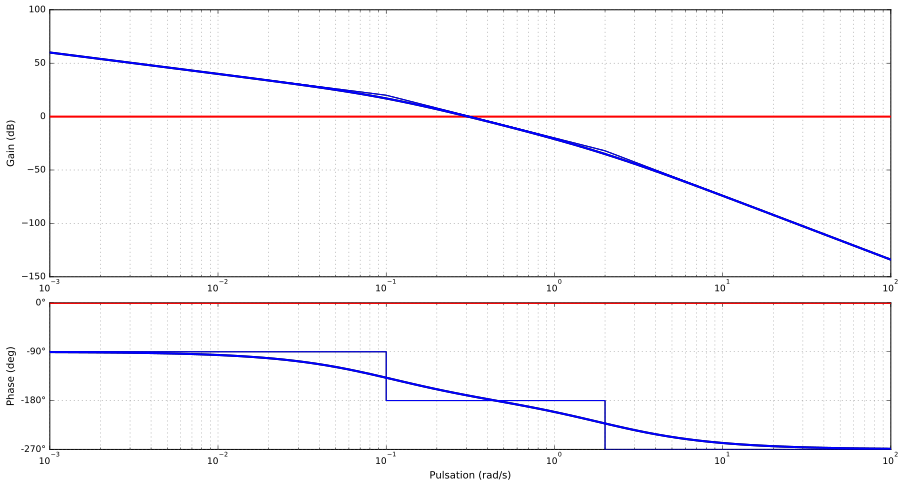
\includegraphics[width=.9\linewidth]{fig_03}

\caption{Architecture maître-esclave \label{fig_03}}
\end{figure}



Une direction automobile découplée doit conserver les qualités d'une direction conventionnelle et
apporter les améliorations de comportement attendues par le conducteur, en termes de performances,
de confort de conduite et de sécurité. Le diagramme (\autoref{ann_01}) précise les principales
exigences.

\subsection*{Modélisation du comportement du système mécanique}

Le modèle utilisé pour la structure est celui de la figure \autoref{fig_09}.

\begin{marginfigure}
\centering
\includegraphics[width=\linewidth]{fig_09}
\caption{Unité de pilotage (chaîne d'énergie) et schéma cinématique  \label{fig_09}}
\end{marginfigure}

Notations :
\begin{itemize}
\item arbre-volant $v$ : le solide constitué du rotor du moteur, de l'arbre volant et du volant ;
\item $G_v$ : centre d'inertie de l'arbre-volant $v$;
\item $\inertie{v}{G_v}$ : opérateur d'inertie de $v$ au point $G_v$;
\item $J_v$ : le moment d'inertie de $v$ autour de l'axe $\axe{G_v}{x_v}$;
\item $f_v$ : le coefficient de frottement visqueux de la liaison pivot ;
\item $\theta_v(t)$ : l'angle de rotation de l'arbre-volant $v$ par rapport au châssis 1 (noté $\theta_v(p)$ dans le
domaine de Laplace) ;
\item $\omega_v(t) $: la vitesse de rotation de l'arbre-volant $v$ par rapport au châssis 1 (noté $\Omega_v(p)$ dans le domaine de Laplace).
\end{itemize}

Hypothèses :
\begin{itemize}
\item le repère lié au châssis 1 est supposé galiléen ;
\item $G_v$ est situé sur l'axe de la liaison pivot ;
\item la liaison pivot est supposée parfaite hormis un couple de frottement visqueux $C_f \vec{x_v}$
;
\item les actions mécaniques du conducteur et du moteur sur l'arbre-volant $v$ se réduisent
respectivement aux couples $C_c \vec{x_v}$ et $C_{\text{mv}} \vec{x_v}$.
\end{itemize}
%
%\question{\label{q5} Après avoir isolé l'arbre-volant $v$ et cité précisément le théorème utilisé, établir l'équation différentielle liant la variable $\theta_v$ et ses dérivées à $J_v$ et aux composantes $C_{\text{mv}}$ et $C_c$ des couples.}
%\ifprof
%\begin{corrige}
%On isole le volant. 
%
%BAME : liaison pivot, frottement visqueux dans la liaison pivot ($C_f = - f_v \dot{\theta}_v(t)$), couple du conducteur et couple moteur. 
%
%Théorème du moment dynamique en projection sur $\vect{x}$ :
%$C_{\text{mv}}(t) + C_c(t) - f_v \dot{\theta}_v(t) = J \dot{\omega}_v(t)$ 
%
%\end{corrige}
%\else
%\fi
%
%
%\question{\label{q6} En supposant les conditions initiales nulles, donner l'expression de la relation précédente dans le domaine de Laplace. Exprimer alors la fonction de transfert$T_v(p)$ telle que
%$\Omega_v(p)=T_v(p)\left[C_c(p)+C_{\text{mv}}(p)\right]$
%sous la forme $T_v(p)=\dfrac{g_v}{1+\tau_v p}$ dont on donnera l'expression de $g_v$
%et $\tau_v$ en fonction de $f_v$ et $J_v$.}
%\ifprof
%\begin{corrige}
%\end{corrige}
%\else
%\fi

\subsection*{Analyse et optimisation du comportement l'unité de pilotage}


Le schéma-blocs retenu est celui de la \autoref{fig_11} où le retour est unitaire. On note $\varepsilon_{\theta v}(t)$ l'écart entre la consigne et l'angle obtenu, et $\varepsilon_{\text{c v}}(t)$ le
couple résultant des couples $C_c$ et $C_{\text{mv}}$.






\begin{figure}[H]
\centering
\includegraphics[width=\linewidth]{fig_11}

\caption{Schéma-blocs de l'unité de pilotage  \label{fig_11}}
\end{figure}


\marginnote{
Pour les applications numériques, on prendra les valeurs suivantes :
$g_v=\SI{5}{rad.s^{-1}.N^{-1}.m^{-1}}$ ; $\tau_v = \SI{0,1}{s}$ et $K_{\text{mv}} = \SI{0,4}{N.m.V^{-1}}$.}

En considérant que la dynamique électromécanique du moteur seul est négligeable devant celle de
l'arbre-volant, on adopte pour la motorisation constituée du moteur à courant continu et de son
électronique de commande, comportant notamment une boucle de courant, un modèle sous la forme
d'un gain pur. On lui associe le gain $K_{\text{mv}}$.


\subsection*{Correction proportionnelle intégrale}

On choisit un correcteur proportionnel intégral (PI) tel que $K_v(p)=K_i \dfrac{1+\tau_i p}{\tau_i p}$
avec $\tau_i =\alpha \tau_v$.



\question{\label{q7} %Justifier brièvement pourquoi un correcteur proportionnel tel que $K_v(p)=K$ ne permet pas de
%satisfaire les critères de précision du cahier des charges, et en quoi le correcteur proportionnel
%intégral assure ou peut assurer la satisfaction de ces critères. 
Quelles sont les conséquences de la
mise en œuvre d'un tel correcteur pour le système, en termes de stabilité ?}
\ifprof
\begin{corrige}
\end{corrige}
\else
\fi


\question{\label{q8} Exprimer la fonction de transfert en boucle ouverte 
$\text{FTBO}_{v1}(p)$ du système corrigé, avec le correcteur PI, telle que $\theta_v(p)=\text{FTBO}_{v1}(p)\varepsilon_{\theta v}(p)$
  sous la forme 
$\text{FTBO}_{v1}(p)=K_{BOv1}\dfrac{1}{p^2}H(p)$ pour
laquelle on précisera les expressions de $K_{\text{BOv1}}$ et de $H(p)$ avec $H(p)$ de gain statique unitaire.
Déduire de cette expression, en le justifiant, si $\alpha$ doit être supérieur ou inférieur à 1 pour que le
système puisse être stabilisé (on pourra donner l'allure du diagramme de phase en fonction de la valeur de $\alpha$).}
\ifprof
\begin{corrige}
\end{corrige}
\else
\fi

On commence par choisir $\tau_i$ en prenant $\alpha=10$ et on cherche à optimiser $K_i$.

%%
On donne 
$\varepsilon_{\theta v}(p)= 
\dfrac{\theta_{\text{v\_ref}}(p)}{1+\text{FTBO}_{\text{v1}}(p)}
-\dfrac{g_v}{p\left(1+\tau_v p\right)}
\cdot \dfrac{C_C(p)}{1+\text{FTBO}_{v1}(p)}$.
%%


\question{\label{q9} Quelle doit être la valeur minimale de $K_i$ pour que les critères de précision soient satisfaits ?}
\ifprof
\begin{corrige}
\end{corrige}
\else
\fi

On donne \autoref{dr_01} le tracé du lieu de transfert de la $\text{FTBO}_{v1}(p)$ dans le plan de Bode, pour $K_i = \SI{0,5}{V.rad^{-1}}$.


\question{\label{q10} Tracer sur le lieu de transfert de la $\text{FTBO}_{v1}(p)$, les diagrammes asymptotiques
dans le plan de Bode. On justifiera rapidement les valeurs particulières de pentes, de pulsations,
de gains et de phases.}
\ifprof
\begin{corrige}
\end{corrige}
\else
\fi

\question{\label{q11} Donner, par lecture du lieu de transfert de la $\text{FTBO}_{v1}(p)$, la valeur de $K_i$ qui permet d'obtenir la
valeur minimale de la marge de phase exigée par le cahier des charges. On donnera cette valeur
pour la pulsation la plus haute dont on précisera la valeur.}
\ifprof
\begin{corrige}
\end{corrige}
\else
\fi

\begin{marginfigure}
On note :
\begin{itemize}
\item $\varphi\left(\omega\right)$ la phase de $H(p)$, soit $\text{Arg}[H(j\omega)]$;
\item $\omega_{\ell}$ la plus grande pulsation qui vérifie $\varphi\left(\omega=\omega_{\ell}\right)=45\degres$.
\end{itemize}
\end{marginfigure}

On donne (\autoref{ann_02}) l'évolution de cette pulsation $\omega_{\ell}$ en fonction de $\alpha$ et un abaque qui représente la valeur maximale $\varphi_m$ de $\varphi\left(\omega\right)$ en fonction de $\alpha$.

\begin{marginfigure}
\centering
\includegraphics[width=\linewidth]{ann_02}

\caption{Abaques de réglage de H(p) en fréquentiel \label{ann_02}}
\end{marginfigure}


\question{\label{q12} Peut-on obtenir la valeur minimale de la pulsation de coupure à \SI{0}{dB} en boucle ouverte, $\omega_0$, fixée au cahier des charges en modifiant la valeur de $\alpha$ et/ou $K_i$ ? On pourra s'aider des abaques fournis
(\autoref{ann_02}) pour justifier la réponse.}
\ifprof
\begin{corrige}
\end{corrige}
\else
\fi

On donne (\autoref{ann_03}), en réponse à un échelon en boucle fermée, les abaques du temps de
réponse à 5\% et du 1\ier dépassement en \% de la valeur finale, en fonction de $K_i$ et pour $\alpha=10$.


\begin{marginfigure}[7cm]
\centering
\includegraphics[width=\linewidth]{ann_03}

\caption{Abaques de réglage en temporel de l'unité de pilotage corrigée \label{ann_03}}
\end{marginfigure}

\question{\label{q13} Conclure sur les capacités de cette correction à satisfaire les critères de l'exigence Id 1-3.3 en
reprenant chaque critère. On rappelle que l'on a choisi $\alpha=10$.}
\ifprof
\begin{corrige}
\end{corrige}
\else
\fi


\subsection*{Correction proportionnelle intégrale et retour tachymétrique}

\begin{figure}[H]
\centering
\includegraphics[width=\linewidth]{fig_12}

\caption{Schéma-blocs de l'unité de pilotage avec retour tachymétrique\label{fig_12}}
\end{figure}


%Q14
\question{\label{q14} Au vu des conclusions de la question précédente, donner deux arguments qui précisent l'objectif poursuivi par la mise en œuvre d'une telle correction.}
\ifprof
\begin{corrige}
\end{corrige}
\else
\fi

%Q15
\question{\label{q15} Exprimer la fonction de transfert en boucle fermée  $T_{\text{vrt}}(p)$ définie par
$\Omega_v(p)=T_{\text{vrt}}(p) \varepsilon_{\text{cv}}(p)$ en
fonction de $T_v (p)$ et $K_{\text{rt}}$. Mettre alors $T_{\text{vrt}}(p)$ sous la forme $T_{\text{vrt}}(p)=T_v(p)\beta \dfrac{1+\tau_v p}{1+\beta \tau_v p}$ pour laquelle, on précisera l'expression de $\beta$ en fonction de $K_{\text{rt}}$ et du gain statique $g_v$.}% défini à la question \autoref{q6}.}
\ifprof
\begin{corrige}
\end{corrige}
\else
\fi

\question{\label{q16} Montrer que la nouvelle fonction de transfert en boucle ouverte $\text{FTBO}_{v2}(p)$, telle que,  $\theta_v(p)=\text{FTBO}_{v2}(p)  \varepsilon_{\theta v}(p) $,
peut ainsi se mettre sous la forme $\text{FTBO}_{v2}(p)=K_{\text{BOv2}} \dfrac{1}{p^2}\dfrac{1+\alpha \tau_v p}{1+\beta \tau_v p}$ pour laquelle on donnera l'expression de $K_{\text{BOv2}}$ en fonction de $K_{\text{mv}}$, $g_v$, $\tau_v$, $K_i$, $\alpha$ et $\beta$.}
\ifprof
\begin{corrige}
\end{corrige}
\else
\fi


On donne sur la \autoref{dr_02} le tracé du lieu de transfert de la $\text{FTBO}_{v2}(p)$ dans le plan de Bode, pour $K_i = \SI{1,2}{V.rad^{-1}}$ (valeur évitant des calculs trop longs), réglé avec
$\beta = 1/6$ (non justifié) et pour $\alpha= 10$ (valeur choisie précédemment).

\question{\label{q17} Justifier que $\beta$ doit être inférieur à 1 pour que la correction par retour tachymétrique soit efficace vis-à-vis du critère de pulsation de coupure à \SI{0}{dB}.}
\ifprof
\begin{corrige}
\end{corrige}
\else
\fi


On donne (\autoref{ann_04}), pour le système en boucle fermée et non perturbé (couple conducteur
nul), les abaques du temps de réponse à 5\% et du premier dépassement en réponse à un échelon
d'angle $\theta_{\text{v\_ref}}$, en fonction de la marge de phase du système, réglé avec $\beta=1/6$.

\begin{marginfigure}
\centering
\includegraphics[width=\linewidth]{ann_04}

\caption{Abaques de réglage en temporel de l'unité de pilotage corrigée avec retour tachymétrique\label{ann_04}}
\end{marginfigure}

\question{\label{q18} Donner par lecture des abaques (\autoref{ann_04}), la valeur de la marge de phase la plus
grande, permettant de satisfaire les deux critères de temps de réponse et de dépassement.}
\ifprof
\begin{corrige}
\end{corrige}
\else
\fi

\question{\label{q19} Déterminer par lecture du lieu de transfert dans le plan de Bode de $\text{FTBO}_{v2}(p)$, tracé dans les
conditions de la question 11,%\ref{q17},
 la valeur de $K_i$ permettant d'obtenir la marge de phase trouvée à la
question précédente.}
\ifprof
\begin{corrige}
\end{corrige}
\else
\fi

\question{\label{q20} Faire une synthèse argumentée de la démarche proposée dans cette partie, pour optimiser le
comportement de l'unité de pilotage.
Conclure, en reprenant chaque critère de l'exigence Id 1-3.3, sur la satisfaction du cahier des
charges}
\ifprof
\begin{corrige}
\end{corrige}
\else
\fi

\question{\label{q21} Avec le réglage établi par le modèle, quel phénomène pourrait endommager certains composants
du système réel ?
Quelle disposition technologique permettrait d'éviter ce phénomène ? Quelles en seraient les
conséquences sur les performances du système ?}
\ifprof
\begin{corrige}
\end{corrige}
\else
\fi


\marginnote{
\footnotesize
\begin{solution}
{\tiny
\begin{enumerate}
\item .
\item $K_{\text{BOv1}}=\dfrac{K_iK_{\text{mv}}g_v}{\alpha \tau_v}$ et $H(p)=\dfrac{1+\alpha \tau_v p}{1+ \tau_v p}$, $\alpha>1$.
\item $K_i \geq 10\alpha \dfrac{\tau_v}{K_{\text{mv}}}$ et $K_i\geq \SI{25}{V.rad^{-1}}$.
\item .
\item $K_i = \SI{5}{V.rad^{-1}}$.
\item .
\item .
\item .
\item $\beta = \dfrac{1}{1+K_{\text{rt}}g_v}$
\item $K_{\text{BOv2}}=\dfrac{K_i K_{\text{mv}}\beta g_v}{\alpha \tau_v}$. %10
\item .
\item $M_{\varphi}=58\degres$.
\item $K_i = \SI{120}{V.rad^{-1}}$. %13
\item .
\item .
\end{enumerate}
}
\end{solution}
\normalsize}

\ifprof
\else
%\begin{marginfigure}[-3cm]
%\centering
\includegraphics[width=3cm]{Cy_02_Ch_01_TD_03_DirectionDecouplee_qr}
%\end{marginfigure}
\fi

\begin{figure}[H]
\centering
%\includegraphics[width=\linewidth]{ann_01}
\includegraphics[width=.8\linewidth]{req_01}
\caption{Exigences \label{ann_01}}
\end{figure}

\begin{figure*}
%\begin{figure}
\includegraphics[height=5cm]{dr_01}
%\caption{Lieu de transfert de $\text{FTBO}_{\text{v1}}(p)$ \label{dr_01}}
%\end{figure}
%\begin{figure}
\includegraphics[height=5cm]{dr_02}
\caption{Lieux de transfert de $\text{FTBO}_{\text{v1}}(p)$ \label{dr_01} et $\text{FTBO}_{\text{v2}}(p)$ \label{dr_02}}
%\end{figure}
\end{figure*}


